% PDF build: pdflatex -> bibtex -> pdflatex
\documentclass[11pt,            % 8, 9, 10, 11 (default), 12, 14, 17, and 20pt
               aspectratio=169, % 43 for 4:3, 169 for 16:9, 1610 for 16:10
               xcolor=svgnames,
               t                % top alignment for vertical alignment
               ]{beamer}

\usepackage{graphicx}
\usepackage{colortbl}
\usepackage[square]{natbib}             % bibliography style package
\usepackage{incgraph}
\usepackage{tikz}
\usepackage{listings}
\usepackage{multimedia}
\usepackage[bahasa]{babel}
\usepackage{amsthm,pifont}
\usepackage{lipsum}

% EDIT file preamble.tex
% EDIT THIS FILE (MIHpreamble.tex)
\lstdefinestyle{CStyle}{
    backgroundcolor=\color{white},
    commentstyle=\itshape\color{DarkGreen},
    keywordstyle=\bfseries\color{red},
    numberstyle=\tiny\color{Gray},
    stringstyle=\color{DodgerBlue},
    basicstyle=\ttfamily,
    breakatwhitespace=false,
    breaklines=true,
    captionpos=b,
    keepspaces=true,
    numbers=left,
    numbersep=5pt,
    showspaces=false,
    showstringspaces=false,
    showtabs=false,
    tabsize=2,
    language=C
}
\lstdefinestyle{PyStyle}{
    backgroundcolor=\color{white},
    commentstyle=\itshape\color{DarkGreen},
    keywordstyle=\bfseries\color{red},
    numberstyle=\tiny\color{Gray},
    stringstyle=\color{DodgerBlue},
    basicstyle=\ttfamily,
    breakatwhitespace=false,
    breaklines=true,
    captionpos=b,
    keepspaces=true,
    numbers=left,
    numbersep=5pt,
    showspaces=false,
    showstringspaces=false,
    showtabs=false,
    tabsize=2,
    language=Python
}
\lstdefinestyle{FortranStyle}{
    backgroundcolor=\color{white},
    commentstyle=\itshape\color{DarkGreen},
    keywordstyle=\bfseries\color{red},
    numberstyle=\tiny\color{Gray},
    stringstyle=\color{DodgerBlue},
    basicstyle=\ttfamily,
    breakatwhitespace=false,
    breaklines=true,
    captionpos=b,
    keepspaces=true,
    numbers=left,
    numbersep=5pt,
    showspaces=false,
    showstringspaces=false,
    showtabs=false,
    tabsize=2,
    language=Fortran
}
\usetikzlibrary{shadows,calc}
\bibpunct{(}{)}{;}{a}{}{,}              % bibliography style format:
%         author [year]
% If you want to use Bahasa Indonesia
\usepackage[bahasa]{babel}
\uselanguage{Bahasa}
\languagepath{Bahasa}
\deftranslation[to=Bahasa]{Theorem}{Teorema}
\deftranslation[to=Bahasa]{Corollary}{Akibat}
\deftranslation[to=Bahasa]{Definition}{Definisi}
\deftranslation[to=Bahasa]{Example}{Contoh}
\deftranslation[to=Bahasa]{Proof}{Bukti}

% ITB COLORS:
\definecolor{ITB}{RGB}{40, 56,144} % note the uppercase RGB
\definecolor{G10}{RGB}{16,116,188} % note the uppercase RGB

\usetheme{Warsaw}
\useoutertheme{infolines,shadow}
\useinnertheme{rounded}
\usefonttheme{professionalfonts,structurebold}
\usecolortheme[named=ITB]{structure}
\setbeamertemplate{items}[ball]                  %default,ball,circle,rectangle
\setbeamertemplate{blocks}[rounded][shadow=true]
\setbeamertemplate{navigation symbols}{}
\setbeamertemplate{theorems}[numbered]
\setbeamertemplate{caption}[numbered]
%\setbeamertemplate{frametitle}[default][left]   %unfortunately, shadow disappear
\setbeamercolor{normal text}{fg=black}
%\setbeamertemplate{background canvas}{\includegraphics
%    [width=\paperwidth,height=\paperheight]{whiteLandscape.jpg}}
\setbeamercovered{transparent}
\usebackgroundtemplate{%
    \begin{tikzpicture}[remember picture,overlay]\node[opacity=0.01,inner sep=0] at (current page.center) {
\includegraphics[scale=0.15]{logoITB}};\end{tikzpicture} % best opacity = 0.025
}
\hypersetup{colorlinks=true,allcolors=FireBrick,bookmarksopenlevel=1}
% \newtheorem{teorema}{Teorema} % theorem environment using Bahasa
% SOME NEW THEOREM/BLOCK ENVIRONMENTS %%%%%%%%%%%%%%%%%%%%%%%%%%%%%%%%%%%%%%%%%%%%
\newtheorem{instance}{Example}
\newcommand*{\theorembreak}{\usebeamertemplate{theorem end}\framebreak\usebeamertemplate{theorem begin}}
% Example or instance %%%%%%%%%%%%%%%%%%%%%%%%%%%%%%%%%%%%%%%%%%%%%%%%%%%%%%%%%%%%
\BeforeBeginEnvironment{instance}{
    \setbeamercolor{block title}{use=example text,fg=white,bg=Brown!50!black}
    \setbeamercolor{block body}{parent=normal text,use=block title example,bg=block title example.bg!10!bg}
}
\AfterEndEnvironment{instance}{
    \setbeamercolor{block title}{use=structure,fg=white,bg=structure.fg!75!black}
    \setbeamercolor{block body}{parent=normal text,use=block title,bg=block title.bg!10!bg}
}
\newtheorem{exercise}{Exercise}
% Exercise %%%%%%%%%%%%%%%%%%%%%%%%%%%%%%%%%%%%%%%%%%%%%%%%%%%%%%%%%%%%%%%%%%%%%%%
\BeforeBeginEnvironment{exercise}{
    \setbeamercolor{block title}{use=example text,fg=white,bg=DarkKhaki!50!black}
    \setbeamercolor{block body}{parent=normal text,use=block title example,bg=block title example.bg!10!bg}
}
\AfterEndEnvironment{exercise}{
    \setbeamercolor{block title}{use=structure,fg=white,bg=structure.fg!75!black}
    \setbeamercolor{block body}{parent=normal text,use=block title,bg=block title.bg!10!bg}
}
\newtheorem{assignment}{Assignment/Homework}
% Exercise %%%%%%%%%%%%%%%%%%%%%%%%%%%%%%%%%%%%%%%%%%%%%%%%%%%%%%%%%%%%%%%%%%%%%%%
\BeforeBeginEnvironment{assignment}{
    \setbeamercolor{block title}{use=example text,fg=white,bg=black}
    \setbeamercolor{block body}{parent=normal text,use=block title example,bg=block title example.bg!10!bg}
}
\AfterEndEnvironment{assignment}{
    \setbeamercolor{block title}{use=structure,fg=white,bg=structure.fg!75!black}
    \setbeamercolor{block body}{parent=normal text,use=block title,bg=block title.bg!10!bg}
}
\newtheorem{algoblock}{Algorithm}
% Example or instance %%%%%%%%%%%%%%%%%%%%%%%%%%%%%%%%%%%%%%%%%%%%%%%%%%%%%%%%%%%%
\BeforeBeginEnvironment{algoblock}{
    \setbeamercolor{block title}{use=example text,fg=white,bg=G10}
    \setbeamercolor{block body}{parent=normal text,use=block title example,bg=block title example.bg!10!bg}
}
\AfterEndEnvironment{algoblock}{
    \setbeamercolor{block title}{use=structure,fg=white,bg=structure.fg!75!black}
    \setbeamercolor{block body}{parent=normal text,use=block title,bg=block title.bg!10!bg}
}
%%%%%%%%%%%%%%%%%%%%%%%%%%%%%%%%%%%%%%%%%%%%%%%%%%%%%%%%%%%%%%%%%%%%%%%%%%%%%%%%%%

% Drop image shadow with gaussian blur (using Tikz, not fancybox) %%%%%%%%%%%%%%%%
% some parameters for customization
\def\shadowshift{3pt,-3pt}
\def\shadowradius{6pt}
\colorlet{innercolor}{black!60}
\colorlet{outercolor}{gray!05}
% this draws a shadow under a rectangle node
\newcommand\drawshadow[1]{
    \begin{pgfonlayer}{shadow}
        \shade[outercolor,inner color=innercolor,outer color=outercolor] ($(#1.south west)+(\shadowshift)+(\shadowradius/2,\shadowradius/2)$) circle (\shadowradius);
        \shade[outercolor,inner color=innercolor,outer color=outercolor] ($(#1.north west)+(\shadowshift)+(\shadowradius/2,-\shadowradius/2)$) circle (\shadowradius);
        \shade[outercolor,inner color=innercolor,outer color=outercolor] ($(#1.south east)+(\shadowshift)+(-\shadowradius/2,\shadowradius/2)$) circle (\shadowradius);
        \shade[outercolor,inner color=innercolor,outer color=outercolor] ($(#1.north east)+(\shadowshift)+(-\shadowradius/2,-\shadowradius/2)$) circle (\shadowradius);
        \shade[top color=innercolor,bottom color=outercolor] ($(#1.south west)+(\shadowshift)+(\shadowradius/2,-\shadowradius/2)$) rectangle ($(#1.south east)+(\shadowshift)+(-\shadowradius/2,\shadowradius/2)$);
        \shade[left color=innercolor,right color=outercolor] ($(#1.south east)+(\shadowshift)+(-\shadowradius/2,\shadowradius/2)$) rectangle ($(#1.north east)+(\shadowshift)+(\shadowradius/2,-\shadowradius/2)$);
        \shade[bottom color=innercolor,top color=outercolor] ($(#1.north west)+(\shadowshift)+(\shadowradius/2,-\shadowradius/2)$) rectangle ($(#1.north east)+(\shadowshift)+(-\shadowradius/2,\shadowradius/2)$);
        \shade[outercolor,right color=innercolor,left color=outercolor] ($(#1.south west)+(\shadowshift)+(-\shadowradius/2,\shadowradius/2)$) rectangle ($(#1.north west)+(\shadowshift)+(\shadowradius/2,-\shadowradius/2)$);
        \filldraw ($(#1.south west)+(\shadowshift)+(\shadowradius/2,\shadowradius/2)$) rectangle ($(#1.north east)+(\shadowshift)-(\shadowradius/2,\shadowradius/2)$);
    \end{pgfonlayer}
}
% create a shadow layer, so that we don't need to worry about overdrawing other things
\pgfdeclarelayer{shadow}
\pgfsetlayers{shadow,main}
\newsavebox\mybox
\newlength\mylen
\newcommand\shadowimage[3][]{%
    \setbox0=\hbox{\includegraphics[#1]{#2}}
    \setlength\mylen{\wd0}
    \ifnum\mylen<\ht0
    \setlength\mylen{\ht0}
    \fi
    \divide \mylen by 120
    \def\shadowshift{\mylen,-\mylen}
    \def\shadowradius{\the\dimexpr\mylen+\mylen+\mylen\relax}
    \begin{figure}
        \begin{tikzpicture}
            \node[anchor=south west,inner sep=0] (image) at (0,0) {\includegraphics[#1]{#2}};
            \drawshadow{image}
        \end{tikzpicture}
        \caption{#3}
\end{figure}}
%%%%%%%%%%%%%%%%%%%%%%%%%%%%%%%%%%%%%%%%%%%%%%%%%%%%%%%%%%%%%%%%%%%%%%%%%%%%%%%%%%

% MAIN BODY  %%%%%%%%%%%%%%%%%%%%%%%%%%%%%%%%%%%%%%%%%%%%%%%%%%%%%%%%%%%%%%%%%%%%%
\begin{document}

% (1a) MIH CUSTOM TITLE STYLE (RECOMMENDED) %%%%%%%%%%%%%%%%%%%%%%%%%%%%%%%%%%%%%%
\title{\LaTeX\ untuk Tugas Akhir}
\subtitle{Sebuah Pengantar}
\author[M I Hakim]{Dr. Muhamad Irfan Hakim}
\titlegraphic{
\includegraphics[width=2cm]{logoITB.png}} % logo as watermark is also provided
\logo{
\includegraphics[scale=0.02]{logoITB}} % logo as watermark is also provided
\institute[FMIPA -- ITB]{Prodi Astronomi\\
    FMIPA -- ITB\\\bigskip
    \textbf{AS4091(2) Tugas Akhir I(II)}}
\date{\number\year}

\setbeamercolor{ITBtitle}{fg=ITB,bg=White}
\makeatletter
\setbeamertemplate{title page}{
    \vbox{}
    \vfill
    \begingroup
    %\centering
    \hfill
    {\usebeamercolor[fg]{titlegraphic}\inserttitlegraphic\par}
    \begin{beamercolorbox}[sep=8pt,right]{ITBtitle} % ITBtitle <--> title
        \usebeamerfont{title}\usebeamercolor[bg]{title}\inserttitle\par%
        \ifx\insertsubtitle\@empty%
        \else%
        \vskip0.25em%
        {\usebeamerfont{subtitle}\usebeamercolor[bg]{subtitle}\insertsubtitle\par}%
        \fi%
    \end{beamercolorbox}%
    \vskip1em\par
    \begin{beamercolorbox}[sep=8pt,right]{author}
        \usebeamerfont{author}\itshape\insertauthor
    \end{beamercolorbox}
    \begin{beamercolorbox}[sep=8pt,right]{institute}
        \usebeamerfont{institute}\insertinstitute
    \end{beamercolorbox}
    \vspace{-1 true cm}
    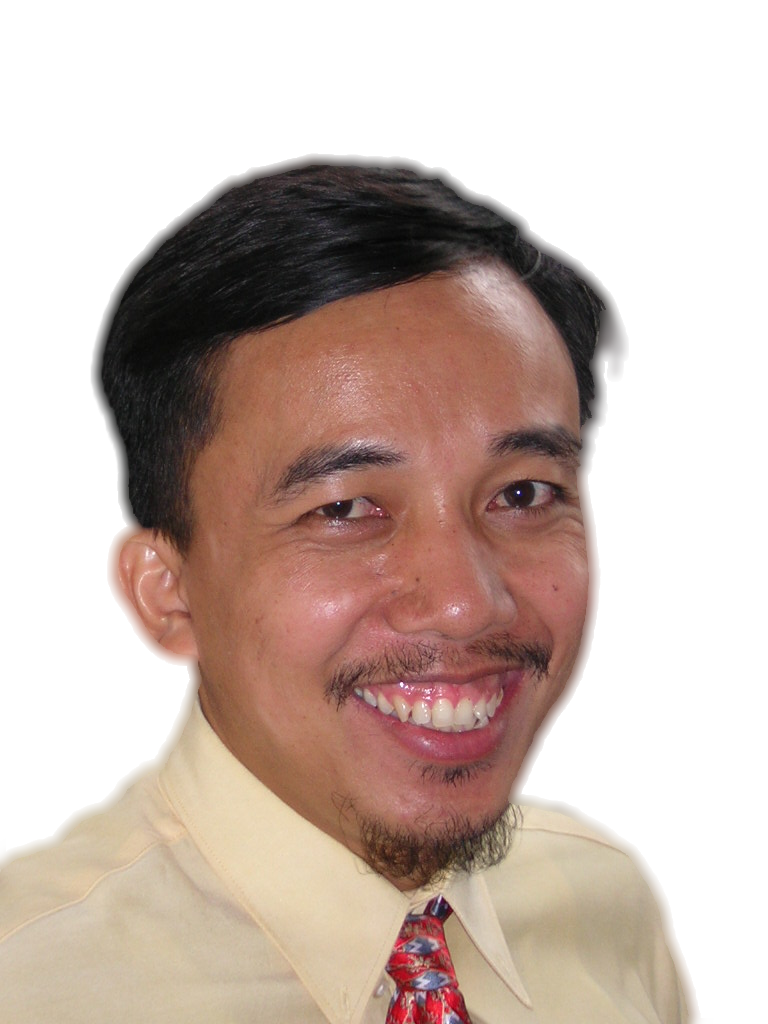
\includegraphics[scale=0.3]{MIHakim-cropped}\hfill\usebeamerfont{date}\insertdate\hspace{8pt}
    \endgroup
    \vfill
}
\makeatother
\begin{frame}[plain,label=home]
\titlepage
\pdfbookmark[0]{Beamer}{home}
\end{frame}
%%%%%%%%%%%%%%%%%%%%%%%%%%%%%%%%%%%%%%%%%%%%%%%%%%%%%%%%%%%%%%%%%%%%%%%%%%%%%%%%%%

% (1b) MIH CUSTOM TITLE STYLE %%%%%%%%%%%%%%%%%%%%%%%%%%%%%%%%%%%%%%%%%%%%%%%%%%%%
%\begin{frame}[plain,label=home]
%\begin{flushright}
%{\Huge\bfseries Beamer}
%
%\vspace{0.25 true cm}
%
%{\LARGE\bfseries Template}
%
%\vspace{0.75 true cm}
%
%{\Large\itshape Dr. Muhamad Irfan Hakim}
%
%\vspace{0.5 true cm}
%
%Astronomy Research Division\\
%FMIPA -- ITB
%
%\bigskip
%
%\textbf{ASnnnn Coursename}
%\end{flushright}
%
%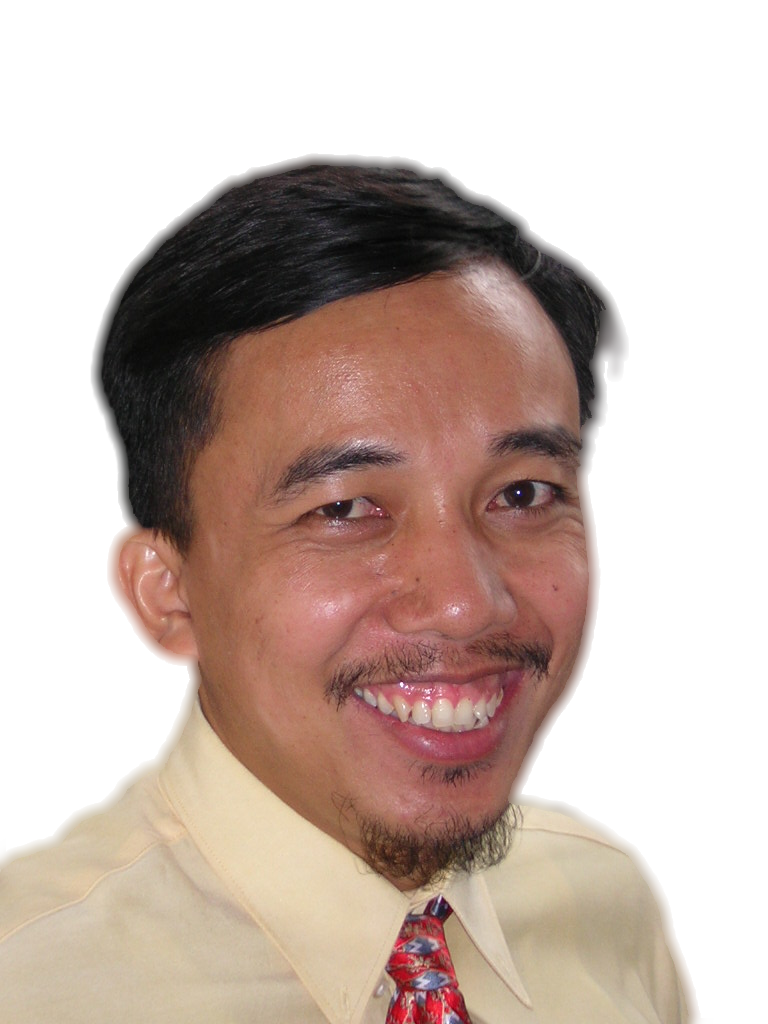
\includegraphics[scale=0.3]{MIHakim-cropped}\hfill{\bfseries\number\year}
%
%\vspace{0.05 true cm}
%
%\hrule
%\pdfbookmark[0]{Beamer}{home}
%\end{frame}
%%%%%%%%%%%%%%%%%%%%%%%%%%%%%%%%%%%%%%%%%%%%%%%%%%%%%%%%%%%%%%%%%%%%%%%%%%%%%%%%%%

% (1c) DEFAULT TITLE STYLE %%%%%%%%%%%%%%%%%%%%%%%%%%%%%%%%%%%%%%%%%%%%%%%%%%%%%%%
%\title{Beamer}
%\subtitle{Template}
%\author[M I Hakim]{\itshape Dr. Muhamad Irfan Hakim}
%\titlegraphic{
%    
\includegraphics[width=2cm]{logoITB.png}
%} % logo as watermark is also provided
%\logo{
\includegraphics[scale=0.02]{logoITB}} % logo as watermark is also provided
%\institute[FMIPA -- ITB]{Astronomy Research Division\\
%                         FMIPA -- ITB\\\bigskip
%                         \textbf{ASnnnn Coursename}}
%\date{\number\year}
%\begin{frame}[plain,label=home]
%\maketitle
%\pdfbookmark[0]{Beamer}{home}
%\end{frame}
%%%%%%%%%%%%%%%%%%%%%%%%%%%%%%%%%%%%%%%%%%%%%%%%%%%%%%%%%%%%%%%%%%%%%%%%%%%%%%%%%%

%%%%%%%%%%%%%%%%%%%%%%%%%%%%%%%%%%%%%%%%%%%%%%%%%%%%%%%%%%%%%%%%%%%%%%%%%%%%%%%%%%
%=======================================================================
\begin{frame}{Disclaimer}
\label{disclaimer}
Struktur materi di slide ini belum dianggap lengkap, dan masih akan diatur ulang dan atau diupdate ke \href{https://github.com/irfan200867/LaTeX-dan-TA-Tesis}{github.com/irfan200867/LaTeX-dan-TA-Tesis}
\pdfbookmark[1]{Disclaimer}{disclaimer}
\end{frame}
%=======================================================================

%=======================================================================
\begin{frame}{Notes}
\label{notes}
--
\pdfbookmark[1]{Notes}{notes}
\end{frame}
%=======================================================================
%%%%%%%%%%%%%%%%%%%%%%%%%%%%%%%%%%%%%%%%%%%%%%%%%%%%%%%%%%%%%%%%%%%%%%%%%%%%%%%%%%

% (2) TABLE OF CONTENTS %%%%%%%%%%%%%%%%%%%%%%%%%%%%%%%%%%%%%%%%%%%%%%%%%%%%%%%%%%
\begin{frame}{\contentsname}
\label{contents}
\tableofcontents
\pdfbookmark[1]{\contentsname}{contents}
\end{frame}
%%%%%%%%%%%%%%%%%%%%%%%%%%%%%%%%%%%%%%%%%%%%%%%%%%%%%%%%%%%%%%%%%%%%%%%%%%%%%%%%%%

\section{Sumber Primer}

\begin{frame}{Sumber Primer \TeX\ , \LaTeX\ dan sekawannya}
\begin{block}{Referensi}
\begin{itemize}
\item \TeX\ \textbf{IS the source}: \href{https://tug.org/}{tug.org}
\item \LaTeX\ adalah salah satu varian turunan dari \TeX
\item TeXLive, MikTeX, \ldots adalah contoh nama-nama untuk kategori distribusi \LaTeX
\item TeXstudio, TeXniccenter, \ldots adalah contoh nama-nama editor \LaTeX
\item Saran saya? Mulailah install \textbf{TeXLive}$+$\textbf{TeXstudio}
\item Bisakah menulis format LaTeX tanpa install? \textbf{Bisa}. Cobalah \href{https://www.overleaf.com}{overleaf.com}
\item Bisakah konversi dari format lain? \textbf{Bisa}. Setelahnya disunting lagi.
\begin{itemize}
    \item Jupyter Notebook: \textit{via} \textbf{jupyter nbconvert} di \underline{Anaconda Prompt}
    \item MS Word (DOCX): \textit{via} \textbf{pandoc}
\end{itemize}
\item \textit{Need help}, \textit{ngoprek}, \textit{custom}: \href{https://tug.org/}{tug.org}, \href{https://www.overleaf.com}{overleaf.com}, TeXstudio LaTeX Reference/User Manual, \href{https://tex.stackexchange.com/}{tex.stackexchange.com}, etc.
\end{itemize}
\end{block}
\end{frame}

\section{Struktur pada Kelas Dokumen}

\begin{frame}{Struktur pada Kelas Dokumen}
\begin{block}{Kelas dan Struktur}
\begin{itemize}
    \item Contoh kelas-kelas: \texttt{article}, \texttt{report}, \texttt{book}, \texttt{beamer} (untuk presentasi)
    \item Struktur dan hirarki:

\bigskip

        \label{hirarki}

    \begin{center}
    \begin{tabular}{|c|l|c|c|c|c|}
    \hline
    \textbf{Urutan} & \textbf{Bagian dokumen} & \texttt{book} & \texttt{report} & \texttt{article} & \texttt{beamer}\\\hline\hline
    1 & \texttt{part} & \ding{51} & \ding{51} & \ding{51} & \\
    2 & \texttt{chapter} & \ding{51} & \ding{51} & & \\
    3 & \texttt{section} & \ding{51} & \ding{51} & \ding{51} & \ding{51}\\
    4 & \texttt{subsection} & \ding{51} & \ding{51} & \ding{51} & \ding{51}\\
    5 & \texttt{subsubsection} & \ding{51} & \ding{51} & \ding{51} & \ding{51}\\\hline
    \end{tabular}
    \end{center}

\end{itemize}

\bigskip

\textbf{Bisa diperiksa di TeXstudio LaTeX Reference/User Manual.}

\end{block}
\end{frame}

\section{Strategi Draft Laporan TA/Tesis \& Presentasi}

\begin{frame}{Strategi Draft Laporan TA/Tesis \& Presentasi dalam \texttt{beamer}}
\begin{block}{Saran}
\begin{enumerate}
\item Teruskan saja dulu \textit{menulis dengan piranti paling dikuasai}\label{nulisAja}
\item \textit{Pahami struktur dasar} dokumen TA/Tesis versi \LaTeX
\item Bila langkah~(\ref{nulisAja}) tidak dalam \LaTeX, \textit{konversikan} ke \LaTeX\ \textit{saat
      sudah dianggap selesai}
\item \textit{Sunting sesuai dengan standard} dokumen \LaTeX\ dan TA/Tesis, termasuk bibliografi.
\item \textbf{Konversi ke PDF} \textit{via} \texttt{pdflatex} dan \texttt{bibtex}, yaitu:
      \texttt{pdflatex} $ \rightarrow $ \texttt{bibtex} $ \rightarrow $ \texttt{pdflatex}
\item \textbf{Ekstrak isi dokumen} \LaTeX\ \textbf{hanya pada bagian-bagian penting} dan menjadi \textit{etalase} TA/Tesis, serta \textit{\bfseries downgrade} \textbf{hirarkinya mengikuti standard }\texttt{beamer} (lihat halaman~\pageref{hirarki})
\end{enumerate}
\end{block}
\end{frame}

\begin{frame}[plain]
    \vfill
    \centering{\Huge\bfseries Now, \LaTeX\ \ldots}
    \vfill
\end{frame}

\section{Enam Tanda Baca Terpenting}

\begin{frame}
\begin{block}{Enam Tanda Baca Terpenting}
\bigskip

\centering{\hspace{0.2cm}$\backslash$\hfill\%\hfill\{\hfill\}\hfill\ [\hfill\ ]\hspace{0.2cm}}

\bigskip
\end{block}

\begin{block}{Peruntukkannya}
\bigskip

``$ \backslash $'' untuk \textit{conserved word} (misal perintah, parameter) di \TeX\ atau \LaTeX. Sebagian perintah \TeX/\LaTeX\ khusus hanya untuk \textbf{MODA TEKS} atau \textbf{MODA MATEMATIKA}.

\bigskip

``\%'' untuk mencegah agar apapun \textbf{di sebelah kanannya tidak dieksekusi} \TeX\ atau \LaTeX.

\bigskip

``\{'' dan ``\}'' untuk penanda blok \textbf{argumen wajib}

\bigskip

``['' dan ``]'' untuk penanda blok \textbf{argumen opsional}

\bigskip
\end{block}

\end{frame}

\section{Penanda Block/Environment}

\begin{frame}[containsverbatim]{Penanda Block/Environment}
\begin{block}{Penanda Block/Environment pada \LaTeX}
\begin{verbatim}
$  ... $           % untuk satu ekspresi matematika DI DALAM PARAGRAF
\[ ... \]          % untuk satu ekspresi matematika/rumus tanpa nomor
   \begin{equation}
    ...            % untuk satu rumus bernomor
   \end{equation}

\begin{equation*}
    ...            % untuk satu rumus tak bernomor
\end{equation*}

\begin{eqnarray}
    ...            % untuk rangkaian baris rumus
\end{eqnarray}
\end{verbatim}
\end{block}

\end{frame}

\begin{frame}[containsverbatim]{Penanda Block/Environment}

    \begin{block}{Penanda Block/Environment pada \LaTeX}
        \begin{verbatim}
            \begin{figure}
                ...            % untuk sisip gambar
            \end{figure}

            \begin{table}
                ...            % untuk menyusun tabel + caption
            \end{table}

            \begin{tabular}{|c|c|}
                ...            % contoh desain tabel 2 kolom rapat tengah
            \end{tabular}
        \end{verbatim}
    \end{block}
\ldots\textbf{dan seterusnya} (editor \LaTeX\ yang baik dapat memandu pilihan \textit{environment}) \ldots
\end{frame}

%%%%%%%%%%%%%%%%%%%%%%%%%%%%%%%%%%%%%%%%%%%%%%%%%%%%%%%%%%%%%%%%%%%%%%%%%%%%%%%%%%
\section{Matematika}
%=======================================================================
\begin{frame}[containsverbatim,allowframebreaks]{Matematika}
\label{math}

Ekspresi matematika $\int x dx$  (ditulis \verb|$\int x dx$|) bergabung dengan naskah dalam satu paragraf.

\bigskip

Sebaris persamaan tak bernomor (terpisah dari paragraf):

\[ \alpha + \beta = 1 \]

\begin{block}{}
\begin{verbatim}
                      \[ \alpha + \beta = 1 \]
\end{verbatim}
\end{block}
\newpage
Sebaris persamaan bernomor (terpisah dari paragraf):

\begin{equation}
\label{sqrtpi}
\int_{-\infty}^{\infty} e^{-x^2} \, dx = \sqrt{\pi}
\end{equation}

\begin{block}{}
\begin{verbatim}
\begin{equation}
\label{sqrtpi}
\int_{-\infty}^{\infty} e^{-x^2} \, dx = \sqrt{\pi}
\end{equation}
\end{verbatim}
\end{block}
\newpage
Barisan persamaan (bernomor dan tak bernomor, terpisah dari paragraf):

\begin{eqnarray}
\sin^2\,x + \cos^2\,x &=& 1\\
(a + b)^2             &=& a^2 + 2ab + b^2\nonumber\\
\alpha &=& \beta + \delta
\end{eqnarray}

\begin{block}{}
\begin{verbatim}
\begin{eqnarray}
\sin^2\,x + \cos^2\,x &=& 1\\
(a + b)^2             &=& a^2 + 2ab + b^2\nonumber\\
\alpha &=& \beta + \delta
\end{eqnarray}
\end{verbatim}
\end{block}

\newpage

Barisan persamaan tak bernomor dan terpisah dari paragraf:

\begin{eqnarray*}
\sin^2\,x + \cos^2\,x &=& 1\\
(a + b)^2             &=& a^2 + 2ab + b^2\\
\alpha &=& \beta + \delta
\end{eqnarray*}

\begin{block}{}
\begin{verbatim}
\begin{eqnarray*}
\sin^2\,x + \cos^2\,x &=& 1\\
(a + b)^2             &=& a^2 + 2ab + b^2\\
\alpha &=& \beta + \delta
\end{eqnarray*}
\end{verbatim}
\end{block}

\end{frame}
%=======================================================================
%%%%%%%%%%%%%%%%%%%%%%%%%%%%%%%%%%%%%%%%%%%%%%%%%%%%%%%%%%%%%%%%%%%%%%%%%%%%%%%%%%

%%%%%%%%%%%%%%%%%%%%%%%%%%%%%%%%%%%%%%%%%%%%%%%%%%%%%%%%%%%%%%%%%%%%%%%%%%%%%%%%%%
\section{Daftar (List)}
%=======================================================================
\begin{frame}[containsverbatim,allowframebreaks]{Daftar (List)}
\label{list}

Daftar tak bernomor urut (\textit{itemized list}):

\begin{itemize}
\item itemized item 1
\item itemized item 2
\item itemized item 3
\end{itemize}

\begin{block}{}
\begin{verbatim}
\begin{itemize}
\item itemized item 1
\item itemized item 2
\item itemized item 3
\end{itemize}
\end{verbatim}
\end{block}
\newpage
Daftar bernomor urut (\textit{enumerated list}):

\begin{enumerate}
\item Three
\item One
\item Two
\end{enumerate}

\begin{block}{}
\begin{verbatim}
\begin{enumerate}
\item Three
\item One
\item Two
\end{enumerate}
\end{verbatim}
\end{block}

\end{frame}
%=======================================================================
%%%%%%%%%%%%%%%%%%%%%%%%%%%%%%%%%%%%%%%%%%%%%%%%%%%%%%%%%%%%%%%%%%%%%%%%%%%%%%%%%%

%%%%%%%%%%%%%%%%%%%%%%%%%%%%%%%%%%%%%%%%%%%%%%%%%%%%%%%%%%%%%%%%%%%%%%%%%%%%%%%%%%
%\section{Transisi Salindia}
%=======================================================================
%\begin{frame}{Transisi Salindia}
%% transblindshorizontal/vertical, transboxin/out, transdissolve, transglitter
%% transslipverticalin/out, transhorizontalin/out, transwipe, transduration{2}
%\pause
%\transboxin<1>
%Frame Body Text (transboxin). \pause\transboxout<2>Frame Body Text (transboxout).
%
%\pause\transblindshorizontal<3>Frame Body Text (transblindshorizontal).
%\pause\transblindsvertical<4>Frame Body Text (transblindsvertical).
%\pause\transdissolve<5>Frame Body Text (transdissolve).
%\pause\transglitter<6>Frame Body Text (transglitter). etc.
%\end{frame}
%=======================================================================
%%%%%%%%%%%%%%%%%%%%%%%%%%%%%%%%%%%%%%%%%%%%%%%%%%%%%%%%%%%%%%%%%%%%%%%%%%%%%%%%%%

%%%%%%%%%%%%%%%%%%%%%%%%%%%%%%%%%%%%%%%%%%%%%%%%%%%%%%%%%%%%%%%%%%%%%%%%%%%%%%%%%%
\section{Gambar}
%=======================================================================
\begin{frame}[containsverbatim,allowframebreaks]{Gambar}

\begin{figure}
\begin{center}
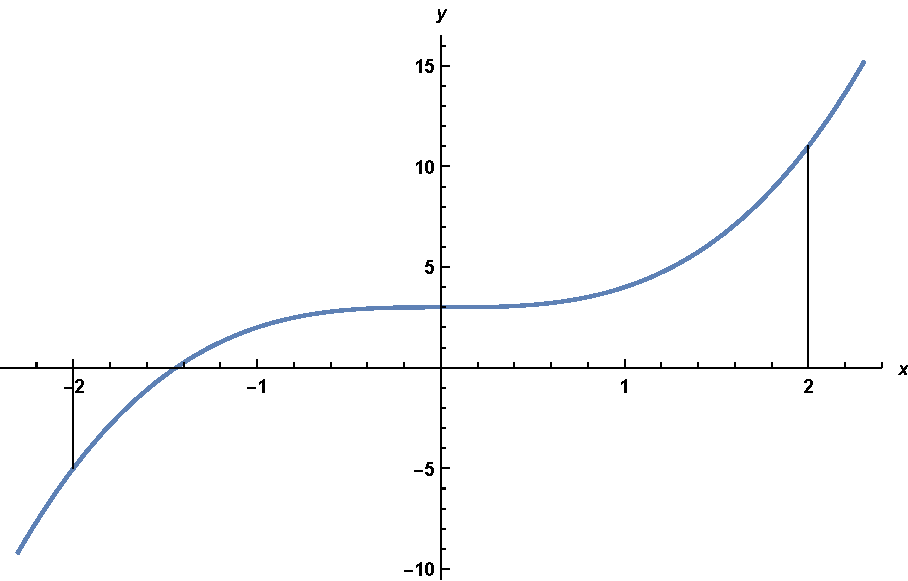
\includegraphics[height=.65\textheight]{plotwithMath.pdf}
%\includegraphics<3>[height=.7\textheight]{whiteLandscape.jpg}
\end{center}
\caption{Gambar vektor (format EPS atau PDF).}
\end{figure}

\begin{block}{}
\begin{verbatim}
\begin{figure}
\begin{center}
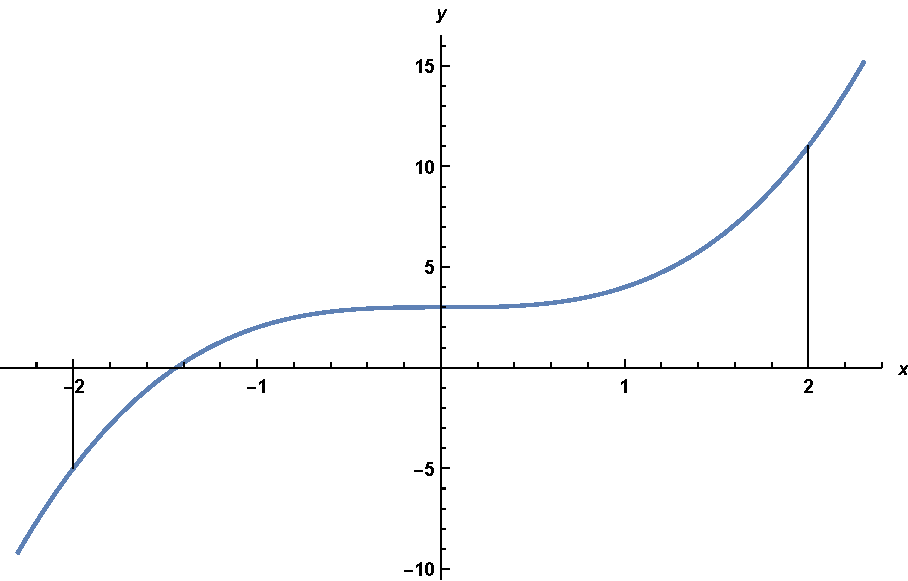
\includegraphics[height=.65\textheight]{plotwithMath.pdf}
\end{center}
\caption{Gambar vektor (format EPS atau PDF).}
\end{figure}
\end{verbatim}
\end{block}

\begin{figure}
\begin{center}
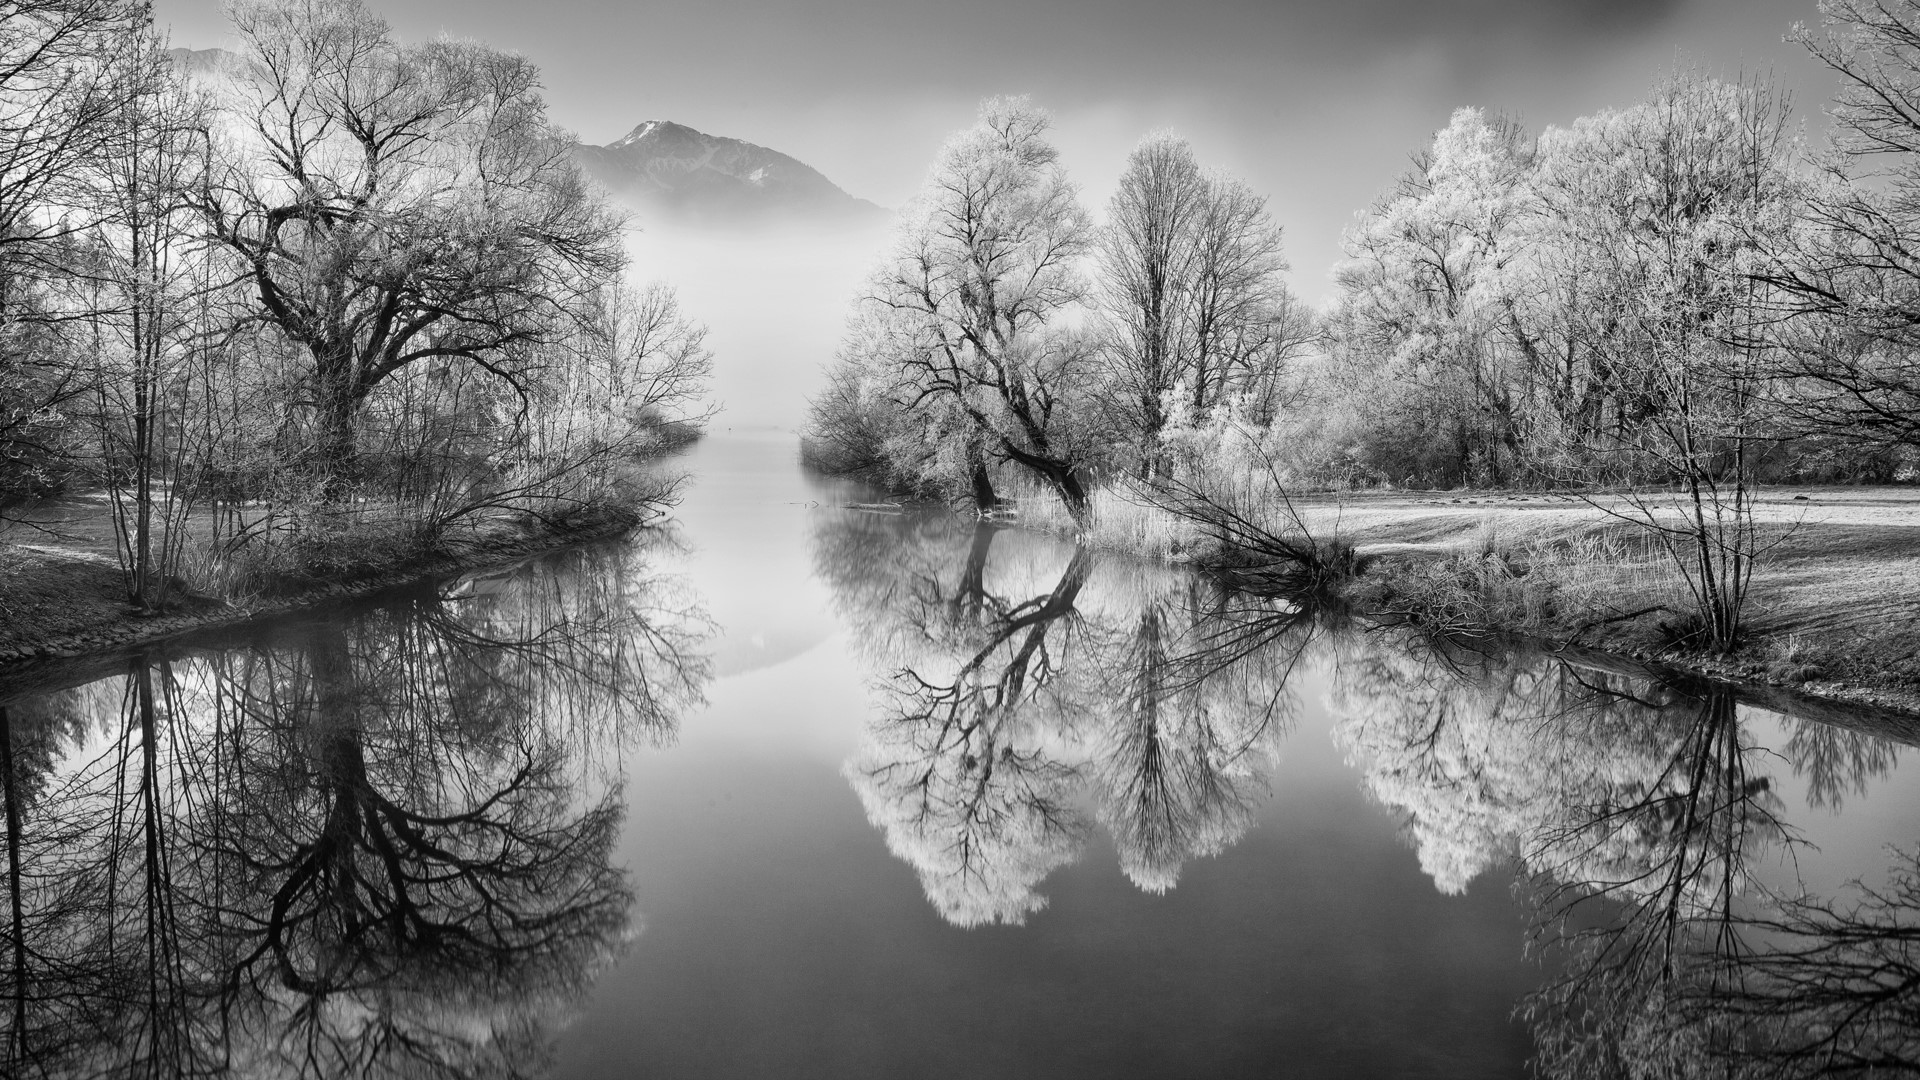
\includegraphics[height=.65\textheight]{whiteLandscape.jpg}
\end{center}
\caption{Gambar \textit{raster} (misal format JPG atau PNG).}
\end{figure}

\begin{block}{}
\begin{verbatim}
\begin{figure}
\begin{center}
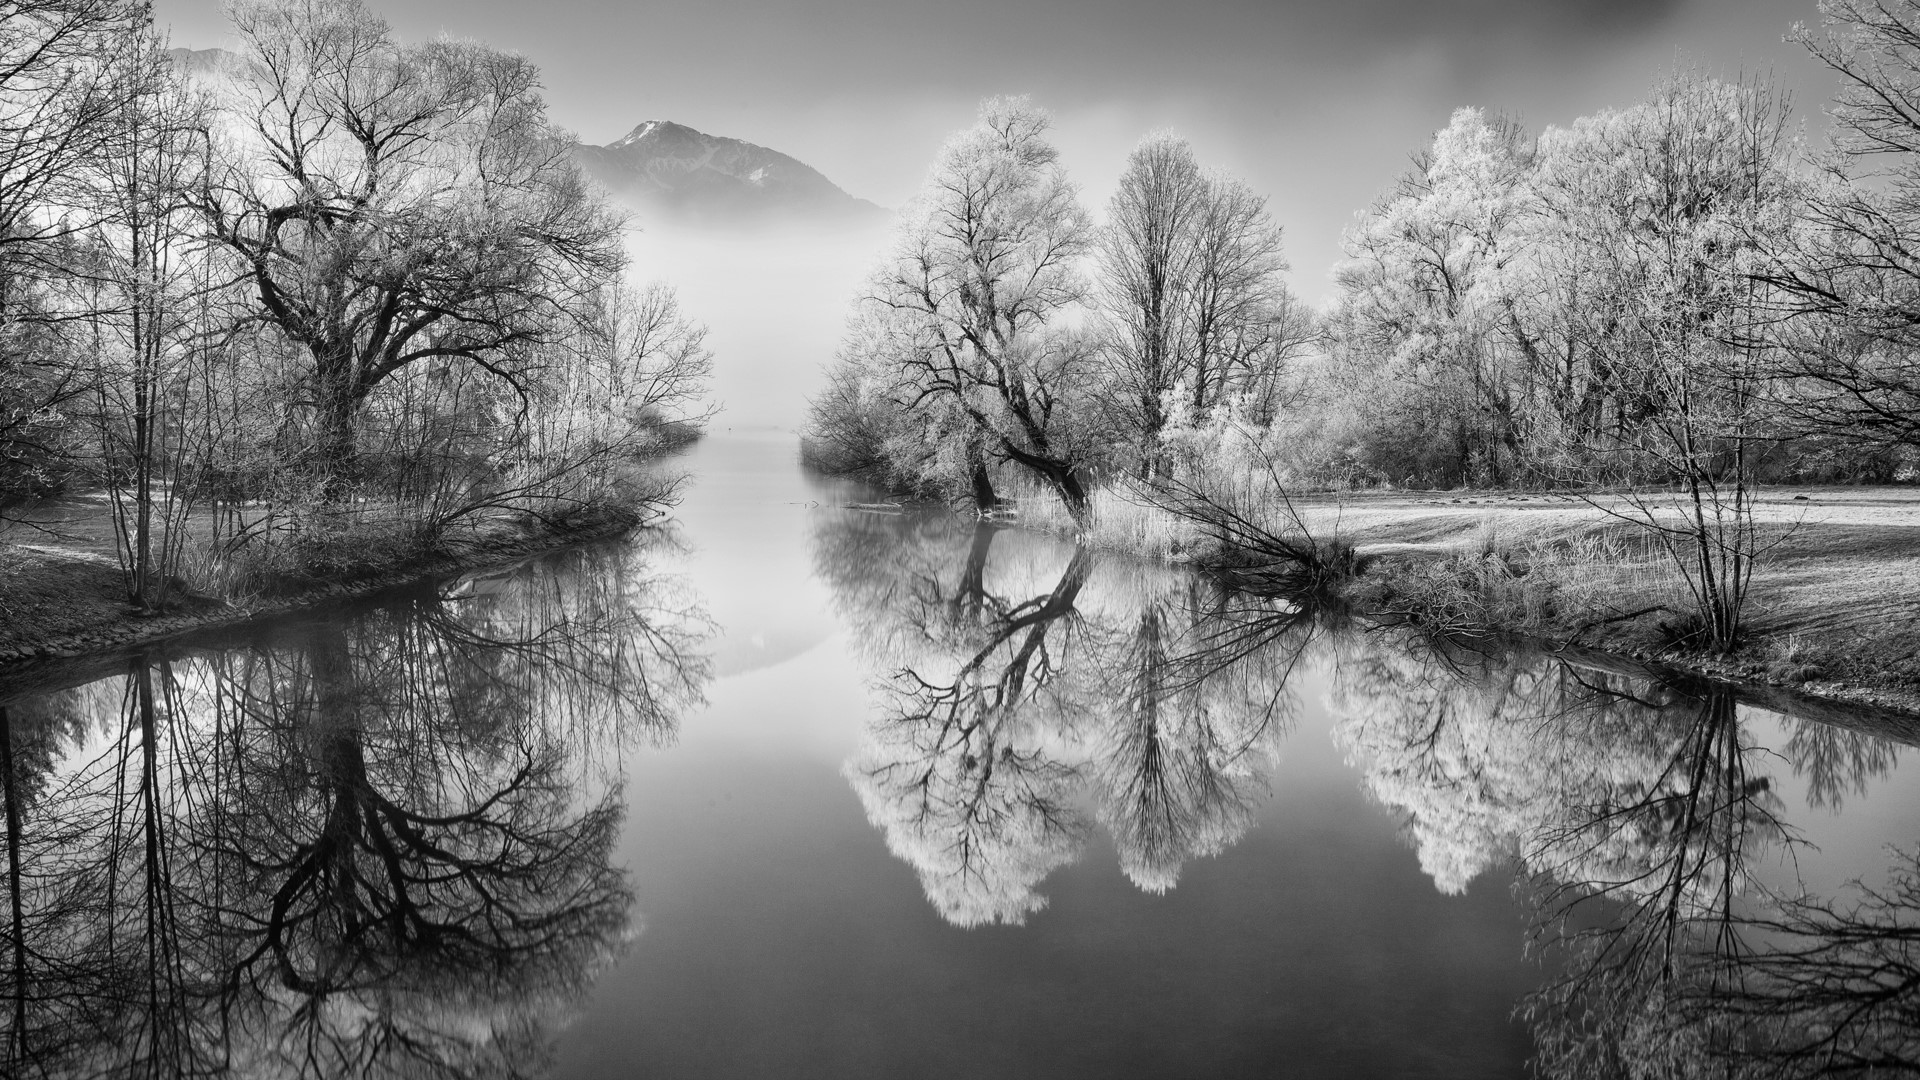
\includegraphics[height=.65\textheight]{whiteLandscape.jpg}
\end{center}
\caption{Gambar \textit{raster} (misal format JPG atau PNG).}
\end{figure}
\end{verbatim}
\end{block}

\end{frame}
%=======================================================================
%%%%%%%%%%%%%%%%%%%%%%%%%%%%%%%%%%%%%%%%%%%%%%%%%%%%%%%%%%%%%%%%%%%%%%%%%%%%%%%%%%

%%%%%%%%%%%%%%%%%%%%%%%%%%%%%%%%%%%%%%%%%%%%%%%%%%%%%%%%%%%%%%%%%%%%%%%%%%%%%%%%%%
%\section{Teorema}
%=======================================================================
%\begin{frame}[allowframebreaks]{Teorema}
%\label{theorem}
%\begin{theorem}
%In a right triangle, the square of hypotenuse equals
%the sum of squares of two other sides.
%\end{theorem}
%
%\begin{block}{Blok dengan judul manasuka}
%Test
%\end{block}
%
%\begin{algoblock}[Bisection]
%\begin{enumerate}
%\item Coba
%\item Cobi
%\end{enumerate}
%\end{algoblock}
%
%\begin{instance}
%Coba.
%\end{instance}
%
%\begin{instance}
%Lagi.
%\end{instance}
%
%\begin{exercise}
%Is $ 2 +2 = 4 $?
%\end{exercise}
%
%\begin{assignment}[Deadline: Today $ +\,2 $,  23:59 WIB]
%Prove that $ \sqrt{2} $ is an irrational number.
%\end{assignment}
%
%\begin{exercise}
%\lipsum[1]
%\theorembreak
%\lipsum[2]
%\end{exercise}
%
%\end{frame}
%=======================================================================
%%%%%%%%%%%%%%%%%%%%%%%%%%%%%%%%%%%%%%%%%%%%%%%%%%%%%%%%%%%%%%%%%%%%%%%%%%%%%%%%%%

%%%%%%%%%%%%%%%%%%%%%%%%%%%%%%%%%%%%%%%%%%%%%%%%%%%%%%%%%%%%%%%%%%%%%%%%%%%%%%%%%%
%\section{Salindia Bersambung-sambung}
%=======================================================================
%\begin{frame}[allowframebreaks]{Satu Pasal dalam Banyak Salindia}
%\lipsum
%\end{frame}
%=======================================================================
%%%%%%%%%%%%%%%%%%%%%%%%%%%%%%%%%%%%%%%%%%%%%%%%%%%%%%%%%%%%%%%%%%%%%%%%%%%%%%%%%%

%%%%%%%%%%%%%%%%%%%%%%%%%%%%%%%%%%%%%%%%%%%%%%%%%%%%%%%%%%%%%%%%%%%%%%%%%%%%%%%%%%
\section{Rujukan Internal}
%=======================================================================
\begin{frame}[containsverbatim,allowframebreaks]{Rujukan Internal}
\lipsum[3]

\bigskip

Lihat persamaan~(\ref{sqrtpi}). Untuk rincinya, sila lihat halaman~\ref{math}. Lihat pula Daftar Isi (halaman~\ref{contents}).

\begin{block}{}
\begin{verbatim}
Lihat persamaan~(\ref{sqrtpi}). Untuk rincinya, sila lihat
halaman~\ref{math}. Lihat pula Daftar Isi (halaman~\ref{contents}).
\end{verbatim}
\end{block}
\end{frame}
%=======================================================================
%%%%%%%%%%%%%%%%%%%%%%%%%%%%%%%%%%%%%%%%%%%%%%%%%%%%%%%%%%%%%%%%%%%%%%%%%%%%%%%%%%

%%%%%%%%%%%%%%%%%%%%%%%%%%%%%%%%%%%%%%%%%%%%%%%%%%%%%%%%%%%%%%%%%%%%%%%%%%%%%%%%%%
\section{Tabel}
%=======================================================================
\begin{frame}{Tabel}

\begin{table}
\label{tabExample1}
\caption{Tabel berwarna.}
\begin{center}
\begin{tabular}{cll}
\rowcolor{Brown}\multicolumn{1}{c}{\textcolor{white}{No}} & \multicolumn{1}{c}{\textcolor{white}{Proxy function}} & \multicolumn{1}{c}{\textcolor{white}{Centroid}}\\
\rowcolor{Khaki}1 & Manhattan & median\\
\rowcolor{DarkKhaki}2 & Euclidean & mean
\end{tabular}
\end{center}
\end{table}
\end{frame}

\begin{frame}{Tabel dengan Lapisan Samar}

\begin{table}
\label{tabExample2}
\caption{Tabel dengan lapisan samar.}
\begin{center}
\begin{tabular}{l<{\onslide}!{\vrule}c<{\onslide<2->}c<{\onslide<3->}c<{\onslide<4->}c<{\onslide<5->}c}
\rowcolor{Brown}Class & A & B & C & D \\
\rowcolor{Khaki}X & 1 & 2 & 3 & 4 \\
\rowcolor{DarkKhaki}Y & 3 & 4 & 5 & 6 \\
\rowcolor{Khaki}Z & 5 & 6 & 7 & 8
\end{tabular}
\end{center}
\end{table}

\end{frame}
%=======================================================================
%%%%%%%%%%%%%%%%%%%%%%%%%%%%%%%%%%%%%%%%%%%%%%%%%%%%%%%%%%%%%%%%%%%%%%%%%%%%%%%%%%

%%%%%%%%%%%%%%%%%%%%%%%%%%%%%%%%%%%%%%%%%%%%%%%%%%%%%%%%%%%%%%%%%%%%%%%%%%%%%%%%%%
%\section{Gambar Berbayang Buram Menggunakan Tikz, bukan Fancybox}
%=======================================================================
%\begin{frame}[allowframebreaks]{Gambar Berbayang}
%\shadowimage[width=.61\linewidth]{whiteLandscape.jpg}{Winter. Picture put by \texttt{shadowimage} command (with shadow).}
%\end{frame}
%=======================================================================

%=======================================================================
\begin{frame}[plain]
\pause
\begin{figure}
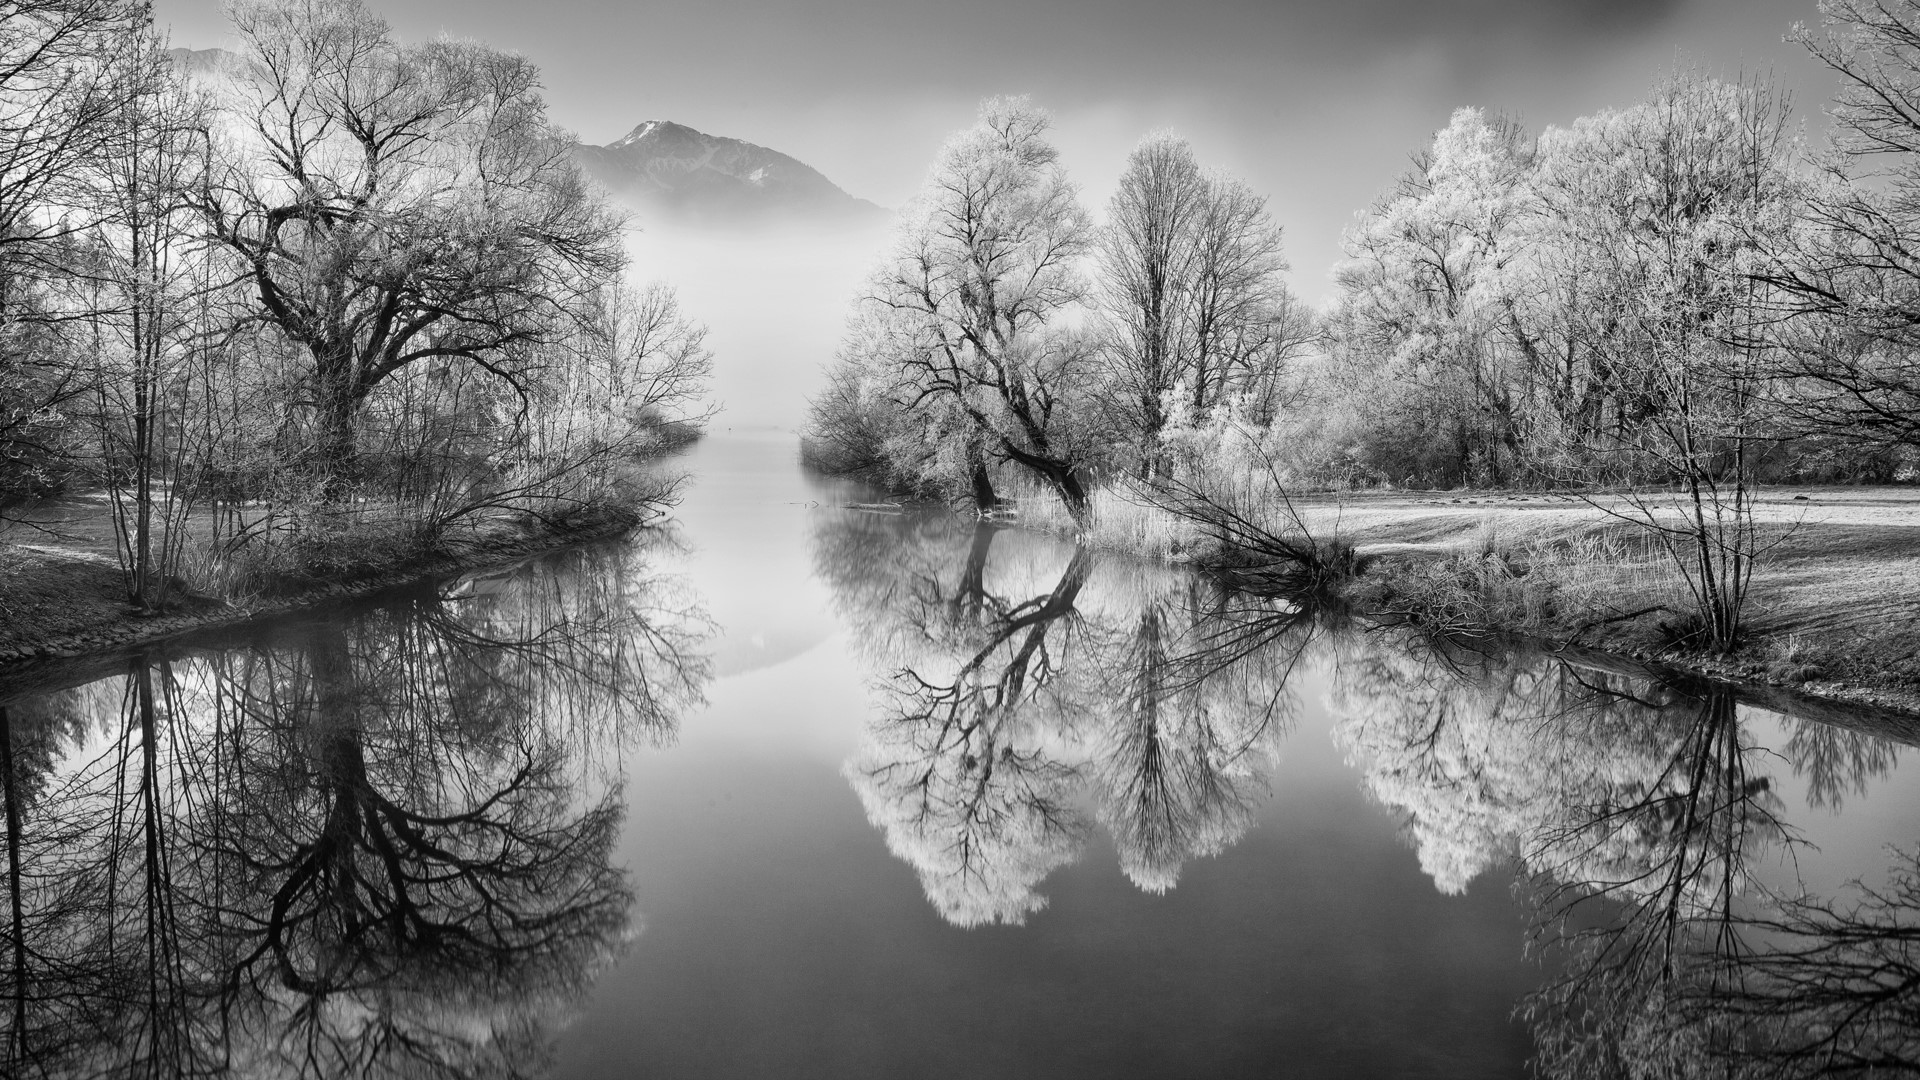
\includegraphics[width=.8\linewidth]{whiteLandscape.jpg}
\pause
\caption{Winter. Picture put by \texttt{figure} environment (without shadow).}
\end{figure}
\end{frame}
%=======================================================================

%=======================================================================
\begin{frame}[plain]
\pause
\shadowimage[width=.7\linewidth]{plotwithMath.pdf}{Plot of $ x^3 + 3 $ with Mathematica.}
\end{frame}
%=======================================================================

%=======================================================================
\begin{frame}[plain]
\incgraph[documentpaper][width=\paperwidth,height=1.05\paperheight]{whiteLandscape.jpg}
\end{frame}
%=======================================================================
%%%%%%%%%%%%%%%%%%%%%%%%%%%%%%%%%%%%%%%%%%%%%%%%%%%%%%%%%%%%%%%%%%%%%%%%%%%%%%%%%%

%%%%%%%%%%%%%%%%%%%%%%%%%%%%%%%%%%%%%%%%%%%%%%%%%%%%%%%%%%%%%%%%%%%%%%%%%%%%%%%%%%
%\section{Dua Kolom}
%=======================================================================
%\begin{frame}[allowframebreaks]{Dua Kolom dalam Satu Salindia}
%
%The line you are reading goes all the way across the slide.
%From the left margin to the right margin.  Now we are going
%to split the slide into two columns.
%
%\begin{columns}[T]
%\begin{column}{0.5\textwidth}
%Here is the first column.  We put an itemized list in it.
%\begin{itemize}
%\item This is an item
%\item This is another item
%\item Yet another item
%\end{itemize}
%\end{column}
%
%\begin{column}{0.45\textwidth}
%\begin{figure}
%\begin{center}
%
\includegraphics[width=0.45\textwidth]{logoITB.png}
%\end{center}
%\caption{Here is the second column.  We will put a picture in it.}
%\end{figure}
%\end{column}
%\end{columns}
%
%The line you are reading goes all the way across the slide.
%From the left margin to the right margin.
%
%\begin{columns}[T]
%\begin{column}{0.5\textwidth}
%Here is the first column.  We put an itemized list in it.
%\begin{itemize}
%\item This is an item
%\item This is another item
%\item Yet another item
%\end{itemize}
%\end{column}
%
%\begin{column}{0.45\textwidth}
%\shadowimage[width=0.75\textwidth]{whiteLandscape.jpg}{Here is the second column.  We will put a picture in it.}
%\end{column}
%\end{columns}
%
%The line you are reading goes all the way across the slide.
%From the left margin to the right margin.
%
%\end{frame}
%=======================================================================
%%%%%%%%%%%%%%%%%%%%%%%%%%%%%%%%%%%%%%%%%%%%%%%%%%%%%%%%%%%%%%%%%%%%%%%%%%%%%%%%%%

%%%%%%%%%%%%%%%%%%%%%%%%%%%%%%%%%%%%%%%%%%%%%%%%%%%%%%%%%%%%%%%%%%%%%%%%%%%%%%%%%%
\section{Sitiran (Citation)}
%=======================================================================
\begin{frame}[containsverbatim,allowframebreaks]{Sitiran (Citation)}
Sitiran ke pustaka rujukan dapat dilakukan, misalnya \cite{siess2000} dan \cite{stepien2002}.

\begin{block}{}
\begin{verbatim}
Sitiran ke pustaka rujukan dapat dilakukan, misalnya \cite{siess2000}
dan \cite{stepien2002}.
\end{verbatim}
\end{block}

\newpage

\begin{block}{Isi file bibliografi (misal bernama `biblio.bib`)}
\begin{verbatim}
@article{siess2000,
    author = {L. Siess and E. Dufour and M. Forestini},
    title = {An Internet Server for Pre-Main Sequence Tracks of Low- and
        Intermediate-mass Stars},
    journal = {A \& A},
    year = {2000}, volume = {358}, pages = {593}}

@article{stepien2002,
    author = {K. St\c{e}pie\'{n}},
    title = {Spin-up of Be Stars in the Pre-Main Sequence Phase},
    journal = {A \& A},
    year = {2002}, volume = {383}, pages = {218}}
\end{verbatim}
\end{block}

\newpage

Dalam dokumen \LaTeX\ ditulis:

\begin{block}{}
\begin{verbatim}
\documentclass{article}
...
\usepackage[square]{natbib}             % bibliography style package
...
\begin{document}
...
\section{Pustaka}     % atau \chapter{Pustaka}

\bibliography{biblio} % karena file bibliografi bernama `biblio.bib`
\bibliographystyle{authordate1}
...
\end{document}
\end{verbatim}
\end{block}

\begin{block}{Tahap kompilasi menuju produksi PDF (yang dianjurkan)}
\begin{itemize}
\item \verb|pdflatex <nama-file-LaTeX.tex>|
\item \verb|bibtex <nama-file-LaTeX>| $\Longleftarrow$ tanpa ekstensi \verb|.tex|
\item \verb|pdflatex <nama-file-LaTeX.tex>|, lalu ulangi
\item \verb|pdflatex <nama-file-LaTeX.tex>|
\end{itemize}
\end{block}

\end{frame}
%=======================================================================
%%%%%%%%%%%%%%%%%%%%%%%%%%%%%%%%%%%%%%%%%%%%%%%%%%%%%%%%%%%%%%%%%%%%%%%%%%%%%%%%%%

%%%%%%%%%%%%%%%%%%%%%%%%%%%%%%%%%%%%%%%%%%%%%%%%%%%%%%%%%%%%%%%%%%%%%%%%%%%%%%%%%%
\section{Coding (verbatim atau listings)}
%=======================================================================
\begin{frame}[containsverbatim,allowframebreaks]{Coding (verbatim atau listings)}
\begin{verbatim}
#include <stdio.h>

/* using verbatim environment */
int main(){
    puts("Hello world!");
    return 0;
}
\end{verbatim}

\begin{lstlisting}[style=CStyle]
#include <stdio.h>

/* using listings package */
int main(){
    puts("Hello world!");
    return 0;
}
\end{lstlisting}

\begin{lstlisting}[style=PyStyle]
# This is python code
def main():
    print('Hello world!')
    return

if __name__ == '__main__':
    main()
\end{lstlisting}

\begin{lstlisting}[style=FortranStyle]
! This is Fortran code
program hello
print *, "Hello world!"
end program hello
\end{lstlisting}

\end{frame}
%=======================================================================
%%%%%%%%%%%%%%%%%%%%%%%%%%%%%%%%%%%%%%%%%%%%%%%%%%%%%%%%%%%%%%%%%%%%%%%%%%%%%%%%%%

%%%%%%%%%%%%%%%%%%%%%%%%%%%%%%%%%%%%%%%%%%%%%%%%%%%%%%%%%%%%%%%%%%%%%%%%%%%%%%%%%%
\section{Video}
%=======================================================================
\begin{frame}{Video (Klik Gambar atau Tulisan)}
\vfill
\centering\movie[autostart,showcontrols,externalviewer]{
\includegraphics[scale=0.2]{generalRelativity.png}}{visualizingGeneralRelativity.mp4}
\vfill
%options: autostart, loop, repeat, palindrome
%options: borderwidth, showcontrols, externalviewer
\end{frame}
%=======================================================================
%%%%%%%%%%%%%%%%%%%%%%%%%%%%%%%%%%%%%%%%%%%%%%%%%%%%%%%%%%%%%%%%%%%%%%%%%%%%%%%%%%

%%%%%%%%%%%%%%%%%%%%%%%%%%%%%%%%%%%%%%%%%%%%%%%%%%%%%%%%%%%%%%%%%%%%%%%%%%%%%%%%%%
\section{Audio}
%=======================================================================
\begin{frame}{Audio (Eksperimental)}
\vfill
\centering\sound[inlinesound,bitspersample=8,channels=2]{WAV Sample}{alarm.wav}
% File types depend on Acrobat Reader versions. Cannot be used with dvips/ps2pdf route
\vfill
%options: autostart, automute, loop, repeat
%options: inlinesound, channels (1), samplingrate (44100), bitspersample (16), encoding
\end{frame}
%=======================================================================
%%%%%%%%%%%%%%%%%%%%%%%%%%%%%%%%%%%%%%%%%%%%%%%%%%%%%%%%%%%%%%%%%%%%%%%%%%%%%%%%%%

%%%%%%%%%%%%%%%%%%%%%%%%%%%%%%%%%%%%%%%%%%%%%%%%%%%%%%%%%%%%%%%%%%%%%%%%%%%%%%%%%%
\section{\refname}
\pdfbookmark[1]{\refname}{references}
%=======================================================================
\begin{frame}{\refname, Untuk Menunjukkan Manfaat File Bibliografi}
\label{references}
\bibliography{biblio}
\bibliographystyle{authordate1}
\end{frame}
%=======================================================================
%%%%%%%%%%%%%%%%%%%%%%%%%%%%%%%%%%%%%%%%%%%%%%%%%%%%%%%%%%%%%%%%%%%%%%%%%%%%%%%%%%

%=======================================================================
%\begin{frame}[allowframebreaks]{Assignment} % or Homework. `allowframebreaks' and
                                             % `theorembreak' for long description
%\begin{frame}{Tugas}                    % or Homework
%\label{assignment}
%\pdfbookmark[1]{Assignment}{assignment} % or Homework
%\begin{assignment}[Deadline: Today $ +\,2 $,  23:59 WIB]
%Prove that $ \sqrt{2} $ is an irrational number.
%%\theorembreak
%%\lipsum[2]
%\end{assignment}
%\end{frame}
%=======================================================================

%=======================================================================
\begin{frame}[plain]
\vfill
\centering{\Huge\bfseries Terima kasih.}

\centering{\hyperlink{home}{\beamerreturnbutton{\bfseries Kembali ke Beranda}}}
\vfill
\end{frame}
%=======================================================================
%%%%%%%%%%%%%%%%%%%%%%%%%%%%%%%%%%%%%%%%%%%%%%%%%%%%%%%%%%%%%%%%%%%%%%%%%%%%%%%%%%

\end{document}
% END OF MAIN BODY %%%%%%%%%%%%%%%%%%%%%%%%%%%%%%%%%%%%%%%%%%%%%%%%%%%%%%%%%%%%%%%
